\documentclass[a4paper,11pt]{article}

\usepackage{préambule}
\usepackage{relsize}
\usetikzlibrary{arrows,positioning,arrows.meta}

\mdfdefinestyle{souvenirstyle}{
    style=greyboxstyle,
    frametitle={Pour s'en souvenir},
}

\newmdenv[style=souvenirstyle]{souvenir}

\begin{document}

Voici une liste de points souvent difficiles à retenir :
\begin{itemize}
	\item \uline{Comparaison des nombre négatifs} : l'ordre des nombres négatifs est “inversé” par rapport au nombres positifs.

	      Par exemple, on a \textbf{-6 > -8}, car 6 < 8.

	      C'est \textbf{aussi} vrai pour les nombres à virgules : on a \textbf{-7,15 < -7,14}, car 7,15 > 7,14.

	      \begin{souvenir}
		      Essaie de placer les nombres sur une droite :

		      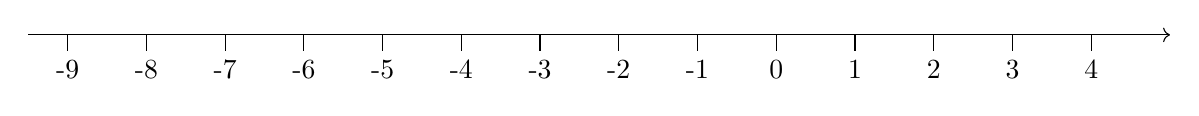
\begin{tikzpicture}
			      \draw[->] (-9.5,0) -- (5,0);
			      \foreach \x in {-9,...,4} {
					      \draw (\x,0) -- ++(0,-0.2) node[below] {\x};
				      }
		      \end{tikzpicture}

		      On voit que \textbf{-6 > -8}.

		      De plus, les nombre négatifs sont en miroir par rapport aux nombre positifs, donc l'ordre est inversé.
	      \end{souvenir}
	\item \uline{L'ordre de l'abscisse et l'ordonnée} : Les coordonnées d'un point du plan sont notées \textbf{(abscisse ; ordonnée)}. L'abscisse est l'axe horizontal (\tikz{\draw[->] (0,0) -- (0.5,0);}), l'ordonnée est l'axe vertical (\tikz{\draw[->] (0,0) -- (0,0.5);}).

	      \begin{souvenir}
		      Les repères sont souvent dessinés ainsi :

		      \begin{tikzpicture}
			      \draw[<->] (0,2) -- (0,0) -- (2,0);
		      \end{tikzpicture}

		      Sur cette figure, l'ordonnée est en \textit{haut}, et l'abscisse en \textit{bas} : ça sonne pareil.
	      \end{souvenir}

	      \begin{souvenir}
		      Avant de voir les repères, on plaçait des points sur des droites horizontales :

		      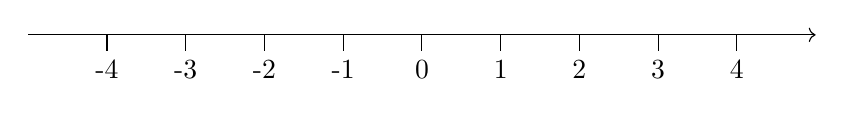
\begin{tikzpicture}
			      \draw[->] (-5,0) -- (5,0);
			      \foreach \x in {-4,...,4} {
					      \draw (\x,0) -- ++(0,-0.2) node[below] {\x};
				      }
		      \end{tikzpicture}

		      C'est donc cette coordonnée qu'on place en premier.
	      \end{souvenir}
	\item \uline{Notation} : Sur le repère suivant

	      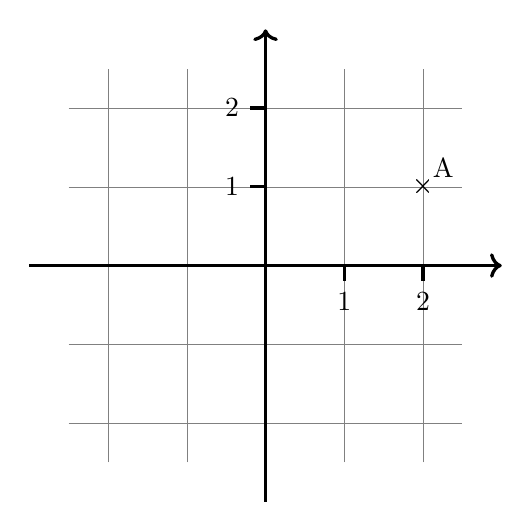
\begin{tikzpicture}
		      \draw[ultra thin,gray] (-2.5,-2.5) grid (2.5,2.5);
		      \draw[very thick,->] (-3,0) -- (3,0);
		      \draw[very thick,->] (0,-3) -- (0,3);

		      \foreach \x in {1,2} {
				      \draw[very thick] (\x,0) -- ++(0,-0.2) node[below] {\x};
				      \draw[very thick] (0,\x) -- ++(-0.2,0) node[left] {\x};
			      }

		      \coordinate (A) at (2,1);
		      \node at (A) {×};
		      \node[above right] at (A) {A};
	      \end{tikzpicture}

	      On note \textbf{A(2 ; 1)}.

	      Les notations A = (2 ; 1), A = 2 ; 1 ou autres ne sont pas valides.
\end{itemize}

\end{document}